% !TeX spellcheck = en_US


\chapter{Experimental Setup}

To experimentally validate the proposed policies, we developed a framework, encompassing a simulation, tools to collect metrics and automatic test runner.
It is based on the Mujoco physics engine, created by Google DeepMind, which provides a realistic simulation of the contact dynamics.
The project is available on GitHub\footnote{\url{...}}.


\section{Swiping Policy}
For the swiping policy, a single whisker executes a sweeping motion over the object.
Performance is quantified by evaluating both the mean absolute error and the standard error in contour reconstruction, with each estimated point $\mathbf{y}_i$ matched to its closest corresponding reference point $\mathbf{x}_i$.

The estimated contour, $C_{\text{est}} = \{\mathbf{y}_i\}_{i=1}^N$, is the set of points obtained by the whisker.
A point is included in the contour only if the whisker is deflected beyond a specified threshold.
The reference contour, $C_{\text{ref}} = \{\mathbf{x}_i\}_{i=1}^N$, consists of points on the object's surface, each being the closest match to the corresponding estimated point.
This reference contour is derived from high-resolution sampling of the object's surface and serves as the ground truth.
The absolute error, defined as $d_i = \|\mathbf{x}_i - \mathbf{y}_i\|$, is the Euclidean (2-norm) distance between the reference and estimated points.

To assess the performance of the swiping policy, we compute the mean absolute error $\bar{d} = \frac{1}{N}\sum_{i=1}^{N} d_i$ and the standard error $\sigma_d = \sqrt{\frac{1}{N-1}\sum_{i=1}^{N} (d_i - \bar{d})^2}$.
The mean absolute error represents the average distance between the reference and estimated points.

Figures~\ref{fig:experiment-disk-swiping}--\ref{fig:experiment-complex-object-swiping} display the results for various objects.
For representation of the estimated contours two colors are used: green if the point error differs from the mean by less than the standard error, and red otherwise.
Which means that red points are the most inaccurate ones, lying in bottom 32 percentile of the error distribution.

\subsection{Contour Estimation of Disk and Rounded Rectangular Box}
Figure~\ref{fig:experiment-disk-swiping} shows the contour estimation of a disk with the swiping policy.
It is the simplest object, and the whisker successfully reconstructs the contour.
It demonstrates a submillimeter accuracy in contour estimation.
No prominent red regions are present, the only ones being random faces of the disk (it's not perfectly round, but rather a polygon).

\begin{figure}[htb]
    \centering
    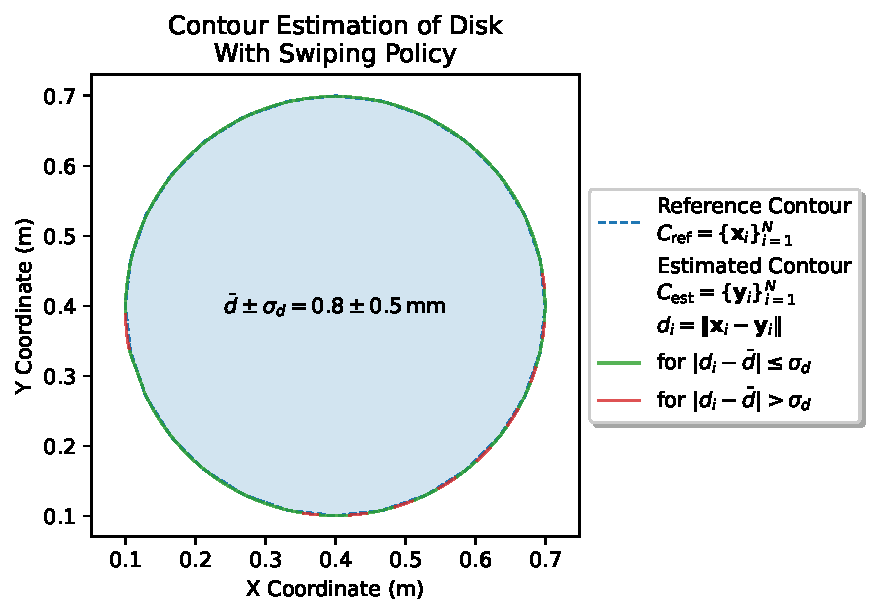
\includegraphics[width=0.8\textwidth]{figures/experiments/disk-swiping}
    \caption{Contour Estimation of Disk With Swiping Policy}
    \label{fig:experiment-disk-swiping}
\end{figure}

Figure~\ref{fig:experiment-rounded-rectangular-box-swiping} illustrates the contour estimation of a rounded rectangular box.
The rectangular box is a more complex object with sharper corners, but it shows a similar level of accuracy and the same mean.

\begin{figure}[htb]
    \centering
    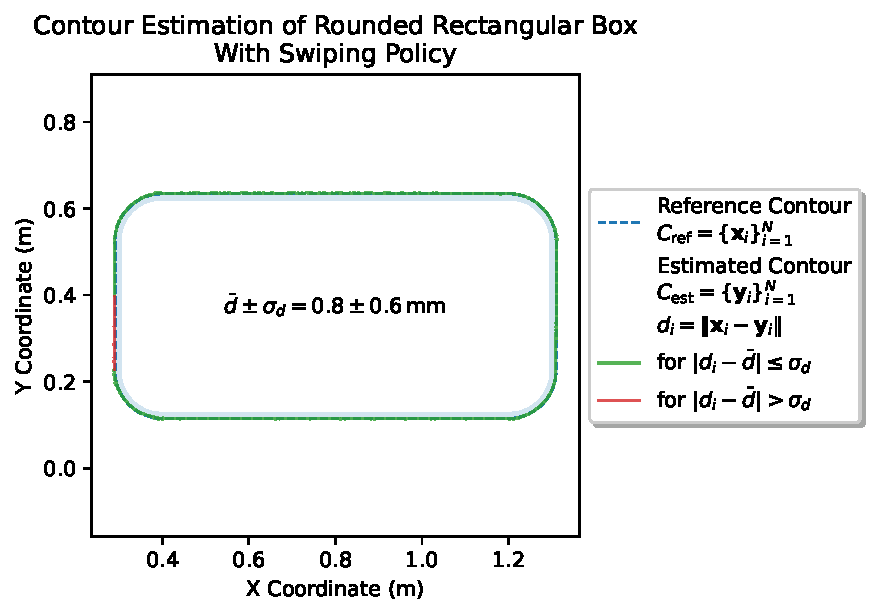
\includegraphics[width=0.8\textwidth]{figures/experiments/rounded-rectangular-box-swiping}
    \caption{Contour Estimation of Rounded Rectangular Box With Swiping Policy}
    \label{fig:experiment-rounded-rectangular-box-swiping}
\end{figure}

\subsection{Contour Estimation of Complex Object}
Figure~\ref{fig:experiment-complex-object-swiping} shows the contour estimation of a complex object.
It has noticable red regions at the inside inflections.
A the inner angles are not smooth, the platform has to quickly adjust to the surface changes, which leads to a higher error rate.
At the first moments the whisker becomes too deflected, and the error increases as the deflection model has worse performance outside of the normal operation range.
The mean error stays at the same level as for disk \ref{fig:experiment-disk-swiping} and rounded rectangular box \ref{fig:experiment-rounded-rectangular-box-swiping}.

\begin{figure}[htb]
    \centering
    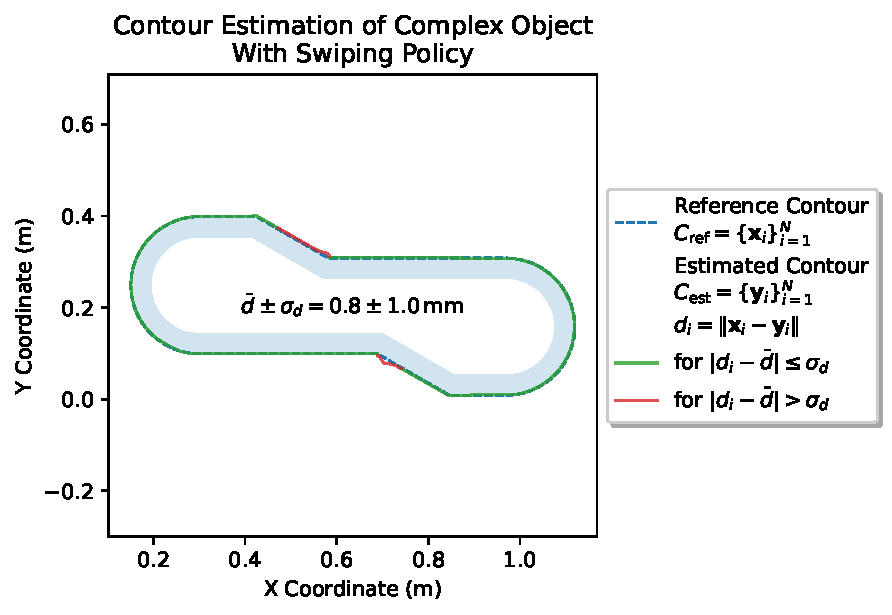
\includegraphics[width=0.8\textwidth]{figures/experiments/complex-object-swiping}
    \caption{Contour Estimation of Complex Object With Swiping Policy}
    \label{fig:experiment-complex-object-swiping}
\end{figure}


\section{Retrieval Policy}
Figures~\ref{fig:experiment-octagon-edges-135deg-swiping-retrieval}--\ref{fig:experiment-wall-edges-90deg-swiping-retrieval} show results for different polygonal objects.

\begin{figure}[htb]
    \centering
    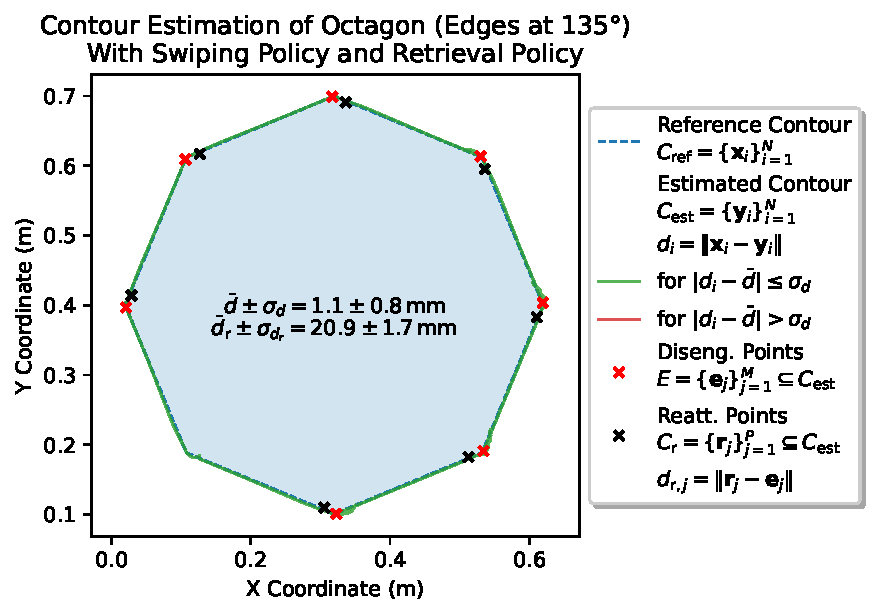
\includegraphics[width=0.8\textwidth]{figures/experiments/octagon-edges-135deg-swiping-retrieval}
    \caption{Contour Estimation of Octagon (Edges at 135°) With Swiping and Retrieval Policy}
    \label{fig:experiment-octagon-edges-135deg-swiping-retrieval}
\end{figure}
\begin{figure}[htb]
    \centering
    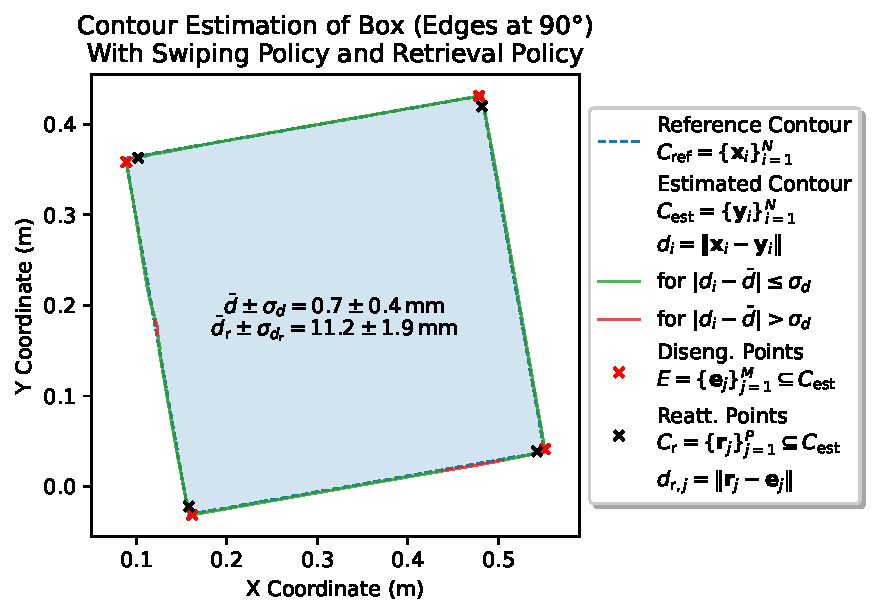
\includegraphics[width=0.8\textwidth]{figures/experiments/box-edges-90deg-swiping-retrieval}
    \caption{Contour Estimation of Box (Edges at 90°) With Swiping and Retrieval Policy}
    \label{fig:experiment-box-edges-90deg-swiping-retrieval}
\end{figure}
\begin{figure}[htb]
    \centering
    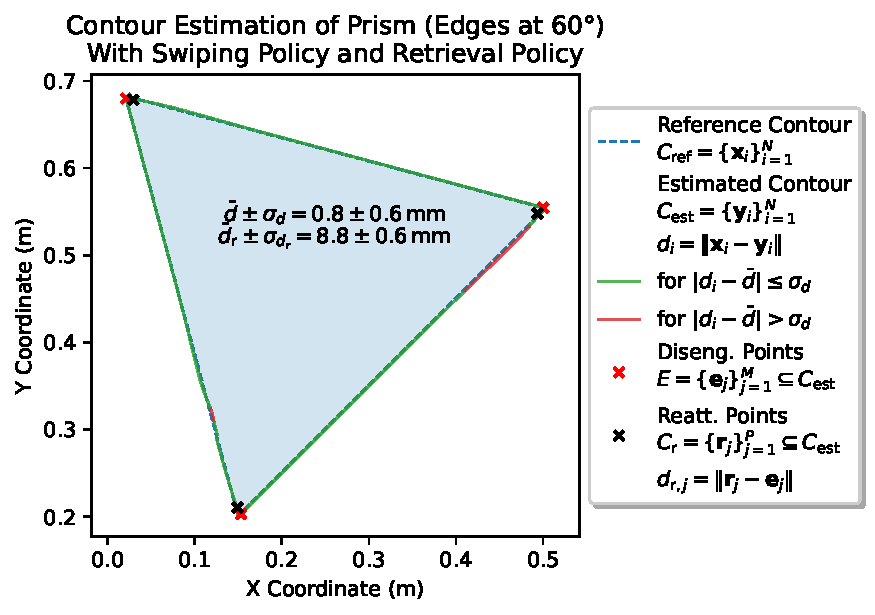
\includegraphics[width=0.8\textwidth]{figures/experiments/prism-edges-60deg-swiping-retrieval}
    \caption{Contour Estimation of Prism (Edges at 60°) With Swiping and Retrieval Policy}
    \label{fig:experiment-prism-edges-60deg-swiping-retrieval}
\end{figure}
\begin{figure}[htb]
    \centering
    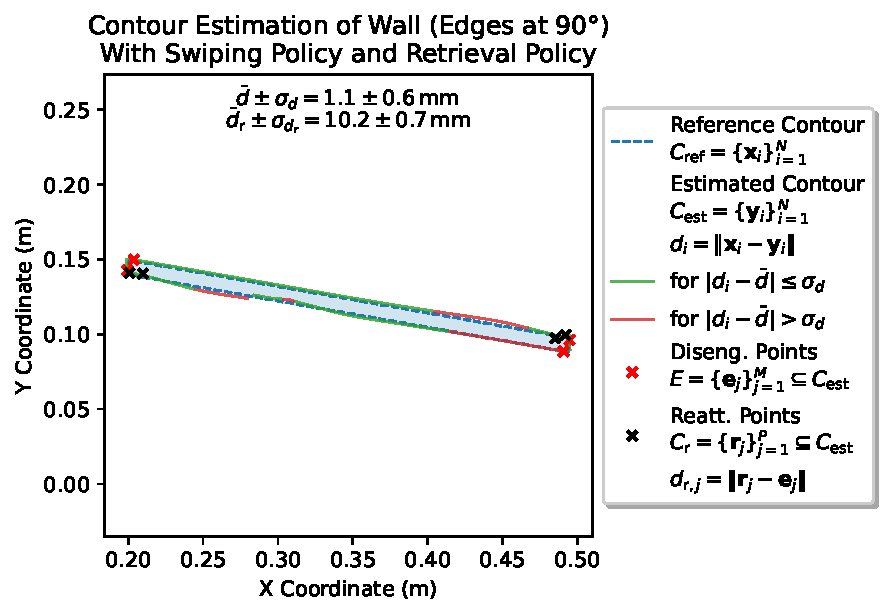
\includegraphics[width=0.8\textwidth]{figures/experiments/wall-edges-90deg-swiping-retrieval}
    \caption{Contour Estimation of Wall (Edges at 90°) With Swiping and Retrieval Policy}
    \label{fig:experiment-wall-edges-90deg-swiping-retrieval}
\end{figure}


\section{Tunneling Policy}
A tunneling approach builds on swiping to navigate confined environments.
Figures~\ref{fig:experiment-smooth-tunnel-swiping-tunneling}--\ref{fig:experiment-round-tunnel-swiping-tunneling} illustrate smooth, zigzag, and round tunnels.

\begin{figure}[htb]
    \centering
    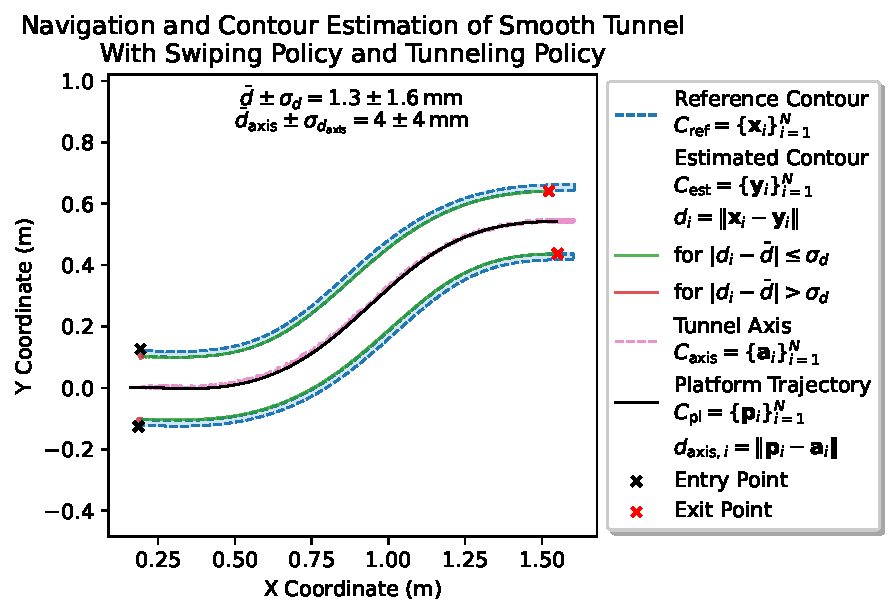
\includegraphics[width=0.8\textwidth]{figures/experiments/smooth-tunnel-swiping-tunneling}
    \caption{Navigation and Contour Estimation of Smooth Tunnel With Swiping and Tunneling Policy}
    \label{fig:experiment-smooth-tunnel-swiping-tunneling}
\end{figure}
\begin{figure}[htb]
    \centering
    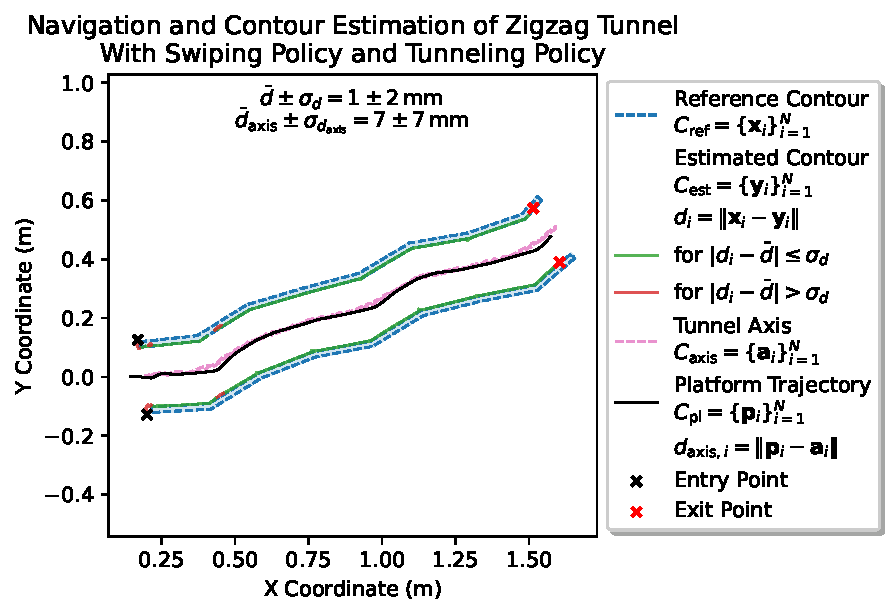
\includegraphics[width=0.8\textwidth]{figures/experiments/zigzag-tunnel-swiping-tunneling}
    \caption{Navigation and Contour Estimation of Zigzag Tunnel With Swiping and Tunneling Policy}
    \label{fig:experiment-zigzag-tunnel-swiping-tunneling}
\end{figure}
\begin{figure}[htb]
    \centering
    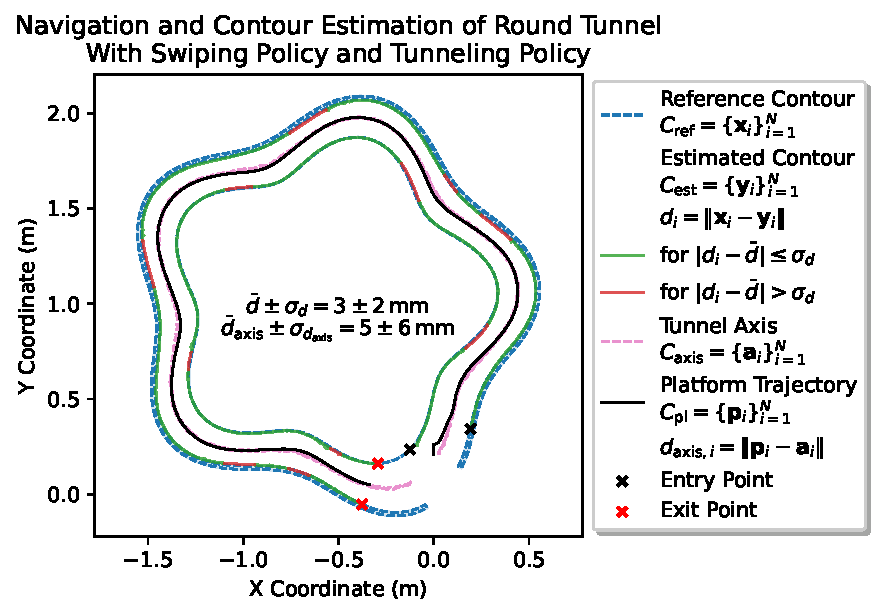
\includegraphics[width=0.8\textwidth]{figures/experiments/round-tunnel-swiping-tunneling}
    \caption{Navigation and Contour Estimation of Round Tunnel With Swiping and Tunneling Policy}
    \label{fig:experiment-round-tunnel-swiping-tunneling}
\end{figure}
